\documentclass[conference]{IEEEtran}
\usepackage[T1]{fontenc}
\usepackage[utf8]{inputenc}
\usepackage{graphicx}
\usepackage{amsmath,amssymb}
\usepackage{array}
\usepackage{url}
\usepackage[hidelinks]{hyperref}
\usepackage{microtype}
\usepackage{balance}
\begin{document}
\title{Reconstructing Sprint-Start Jira State for Leakage-Aware Outcome Prediction}
\author{\IEEEauthorblockN{Hani AbuSharkh}
\IEEEauthorblockA{Higher Colleges of Technology\\Al Ain, UAE\\habusharkh@hct.ac.ae}
\and
\IEEEauthorblockN{Maryam Hanif}
\IEEEauthorblockA{United Arab Emirates University\\Al Ain, UAE\\700052696@uaeu.ac.ae}
\and
\IEEEauthorblockN{Rafat Damseh}
\IEEEauthorblockA{United Arab Emirates University\\Al Ain, UAE\\rdamseh@uaeu.ac.ae}}
\date{}
\maketitle

\begin{abstract}
A present-day Jira export shows how a sprint ended, not what the team knew when it began, so sprint-risk models trained on it can learn from hindsight. For eight open-source TAWOS projects we replay the change log back to the first day of each sprint (2,602 sprints, 1,691 with committed work), log where missing history forces a static fallback, and test planning-time and in-sprint classifiers for late closure and spillover under time-ordered, leave-one-project-out (LOPO) and outside-project splits. Late closure is moderately rankable. Gradient boosting reaches ROC-AUC 0.751 on one time-ordered split and 0.696 $\pm$ 0.054 over five, mostly on the team's own past lateness, and transfers weakly to ten MariaDB and MongoDB projects (mean AUC 0.620, with the interval above chance in two of eight). Spillover, defined as any committed issue left unfinished, is 94\% positive and close to mechanical. The raw count of committed issues ranks it at 0.881, and at mid-sprint the count of committed issues still open scores 0.945, nearly matching gradient boosting with progress features (0.957). Among the leakage checks, shuffling sprints before splitting adds 0.07 to late-closure AUC and two reproduced mistakes inflate F1 by up to 0.24, while restricting history to finished sprints, once separated from the features added with it, does not raise AUC. The contribution is the reconstruction and the audit, not a risk tool.
\end{abstract}

\begin{IEEEkeywords}
Scrum, sprint analytics, Jira, machine learning, explainability, Shapley values, data leakage
\end{IEEEkeywords}

\section{Introduction}

A sprint misses its boundary in two ways that Jira records by itself. It spills over when an issue committed at the start is still unresolved at the planned end, and it closes late when Jira stamps its completion more than a day past that end. Neither is a judgment on the team. We ask whether either can be ranked from what was known on the first day of the sprint, and whether watching the sprint unfold adds anything. To keep hindsight out, every feature is rebuilt only from events time-stamped at or before the point of prediction.

That line is harder to hold than it sounds, because a present-day Jira export is no snapshot of planning day. Issues move between sprints, estimates get revised, and several sprints are usually open at once, so the current issue-to-sprint link cannot tell work committed at planning from work added later. We replay the TAWOS change log back to each sprint's start and record, per project, where a missing history forces a static fallback. A second leak is easier to miss. In 71\% of our sprints the previous sprint had not reached its planned end when the next began, so any summary of it can carry an outcome nobody could have known yet.

This is a data and evaluation contribution, not a deployable risk tool. It consists of a sprint-start reconstruction with an account of how much of it fell back on static values; a leakage-aware evaluation of planning-time classifiers with per-project time splits, LOPO testing, project-cluster bootstrap intervals and outside projects; and, under the same protocol, in-sprint warnings at 25\%, 50\%, 75\% and 100\% of the planned duration. Throughout, we set each model against the simplest rule that could do its job, and two of our own earlier claims did not survive that test. Fig.~\ref{fig:pipeline} lays out the pipeline and Table~\ref{tab:headline} pins each headline result to its model, split, population and comparator. All of it rests on eight open-source projects plus ten outside ones, so we read the numbers as evidence about those projects, not as a general benchmark.

\section{Related Work}

Machine learning on Agile data has mostly chased effort. Story points have been estimated from issue text \cite{r1} and issue fields \cite{r2}, and a TAWOS replication \cite{r3} found simple baselines kept pace once the features were fixed, a pattern we meet again on spillover. Sprint2Vec \cite{r4} regresses delivery on learned sprint embeddings, and Hearty et al. \cite{r5} forecast velocity with a dynamic Bayesian network.

The nearest study is Choetkiertikul et al. \cite{r19}, who predicted the gap between committed and delivered story points for 3,834 iterations of five JIRA projects, MongoDB among them. They rebuilt each iteration's state at the prediction time from the issue change logs, at the start and at 30\%, 50\% and 80\% of the iteration. Our reconstruction follows the same principle, so we do not claim it as new. What we add is an account of where the change log runs out and a static value stands in, the timing of history features when sprints overlap, two binary outcomes with their own populations, comparisons against learning-free counting rules, and reproduced leakage mechanisms. Our search was not systematic. Table~\ref{tab:related} puts these studies side by side.

\begin{table}[!t]
\centering\scriptsize
\caption{The nearest prior work and what this study adds.}
\label{tab:related}
\setlength{\tabcolsep}{3pt}
\begin{tabular}{llll}
\hline
Study & Unit & Target & Prediction-time state\\
\hline
\cite{r1}--\cite{r3} & Issue & Story points & Not applicable\\
\cite{r4} & Sprint & Delivery and quality & Not reported\\
\cite{r5} & Iteration & Velocity & Not reported\\
\cite{r19} & Iteration & Delivered vs.\ committed & Rebuilt (change log)\\
\cite{r7} & Sprint & Performance class & In-sprint burndown\\
\cite{r8} & Sprint & Deliverability & Not reported\\
This work & Sprint & Spillover, late closure & Rebuilt, provenance logged\\
\hline
\end{tabular}
\end{table}

\begin{figure}[t]
\centering
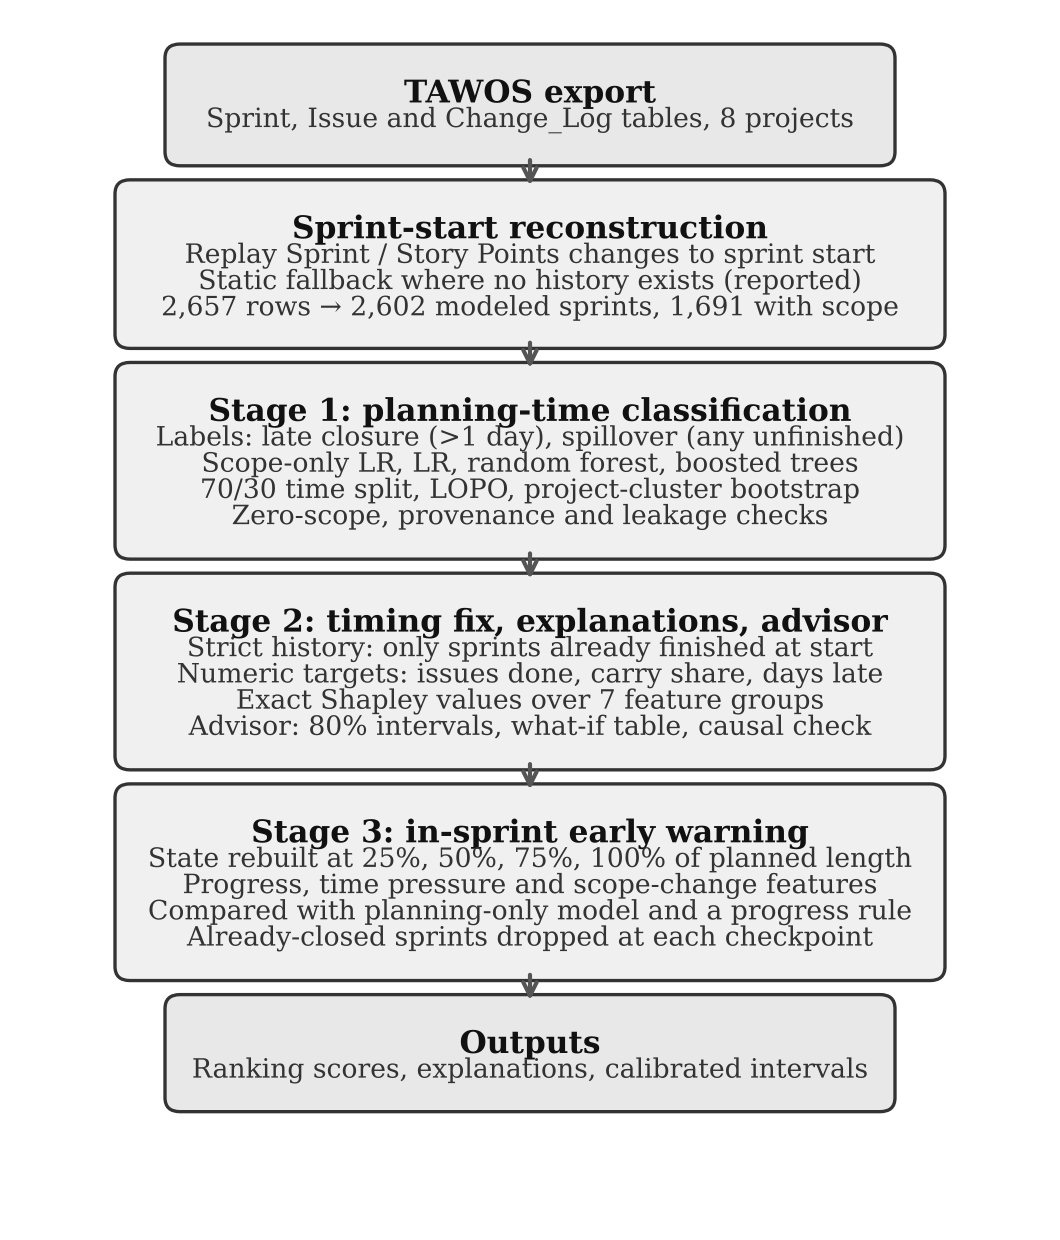
\includegraphics[width=0.75\columnwidth]{fig1_pipeline.png}
\caption{The three-stage pipeline. Every stage uses the same reconstructed cohort, the same per-project time split and the same LOPO folds.}
\label{fig:pipeline}
\end{figure}

Two sprint-level classification studies prompted our leakage checks. Pérez Castillo et al. \cite{r7} classified sprint performance from burndown features visible only while the sprint runs, which makes the task retrospective rather than a forecast. Obike et al. \cite{r8} reported near-perfect deliverability AUC after running SMOTE oversampling \cite{r15}, but without describing a train-test split taken first. We did not read either implementation and make no claim about their published numbers; we reproduce both mechanisms on our own data (Section~\ref{sec:leak}).

For the explanations we take Shapley values from Lundberg and Lee \cite{r9}, but compute them exactly over feature groups, since Jiarpakdee et al. \cite{r11} showed how correlated metrics distort a per-feature reading; Molnar \cite{r10} covers the general case. Our in-sprint setup is a case of outcome-oriented predictive process monitoring \cite{r12}, with its alarm-based extensions \cite{r13}, in which a running case is scored at a sequence of prefixes; \cite{r19} already applied that idea to iterations.

\section{Data and Methods}

\subsection{Dataset and Sprint-Start Reconstruction}

Our data comes from the Sprint, Issue and Change\_Log tables of TAWOS \cite{r6}. We keep the eight open-source Jira projects with at least 30 sprint records apiece: Apache Mesos, Appcelerator Studio, Atlassian Confluence Cloud and Server, LSST Data Management, Mule, Titanium SDK and Titanium Mobile. The export carries 2,657 sprint rows, 145,309 issues and 88,364 change events on the Sprint and Story Points fields. We exclude the 44 sprints still marked FUTURE or ACTIVE and three CLOSED rows that finish before they begin, and drop each project's first eligible sprint as a cold start. That leaves 2,602 modelled sprints.

We rebuild the committed scope rather than read it off the final export. Starting from the latest recorded state, the code walks each issue's Sprint and Story Points changes back to the sprint-start timestamp; an issue counts as committed only if, at that moment, it existed, belonged to the sprint, and had not yet been resolved. That gives 20,603 issue-sprint commitments. When an issue has no recorded change for a field, we fall back on its static value and log it: 7.2\% of commitments lean on the static sprint link and 45.1\% on static story points, and 73.5\% of issues carry no story points at all and count as zero. Coverage is uneven, from 54.1\% of commitments with observed sprint history in Confluence Cloud up to 99.1\% in Confluence Server, so Section~\ref{sec:prov} re-runs the analysis on provenance-restricted subsets.

At the start instant, 911 sprints (35.0\%) hold no committed issue and 1,691 carry real scope. Many of the 911 are not unplanned sprints. In 33\% of them the first issue joins within an hour after the start and in 42\% within a day, so the count partly reflects teams pressing Start before loading the board. We keep the exact start instant as the boundary, since anything later is not planning-time scope, and leave a grace window to future work.

\subsection{Outcomes}

Late closure is 1 when Jira's completion timestamp runs more than a day past the planned end, and is defined for all 2,602 sprints. Spillover is 1 when at least one committed issue is still unresolved at the planned end; we score it only on the 1,691 nonempty sprints, since a sprint that commits nothing cannot spill. The label is 94\% positive, so the spillover test set holds only 29 negatives. Three numeric targets sit alongside the labels: issues completed and carry share (the fraction of committed issues left unfinished) on the nonempty sprints, and days late, capped at 30, on all of them.

\begin{table*}[!t]
\centering\scriptsize
\caption{Study design and headline results. $n$ (positives) is the test denominator of each figure; checkpoint rows count sprints still open. Differences are row model minus comparator, with 95\% project-cluster bootstrap intervals; absolute intervals where the artifact reports them. GB: gradient boosting; RF: random forest; LR: logistic regression; MAE: mean absolute error; SD: standard deviation; SE: standard error; scope only: committed issues, story points and sprint length; strict and legacy name the history feature set. Row 16 trains on TAWOS and tests on MariaDB without story points (SP), with a sprint-level interval; row 17 is mean $\pm$ SD over five time-ordered repeats; row 18 is mean $\pm$ SD across the eight outside projects where late closure can be measured. Rows 19 and 20 use no model.}
\label{tab:headline}
\setlength{\tabcolsep}{2pt}
\begin{tabular}{llllllll}
\hline
 & Task & Split & $n$ (pos.) & Model, features & Result & Difference [95\% CI] & Comparator\\
\hline
1 & Late closure & Time & 786 (246) & GB, strict & AUC .751 & $+$.111 [.028, .258] & Project rate .640\\
2 & Late closure & Time & 786 (246) & GB, strict & AUC .751 & $+$.221 [.098, .369] & Scope-only LR .530\\
3 & Late closure & LOPO & 2,602 (1,006) & RF, strict & AUC .642 & $+$.110 [.018, .215] & Scope-only LR .532\\
4 & Late closure & LOPO & 2,602 (1,006) & RF, legacy & AUC .600 & --- & Per project .531--.780\\
5 & Spillover, nonempty & Time & 511 (482) & LR, scope only & AUC .885 [.818, .922] & $+$.073 [.007, .117] & GB, strict .812\\
6 & Spillover, nonempty & LOPO & 1,691 (1,575) & LR, scope only & AUC .837 & $-$.017 [$-$.051, .007] & LR, strict .854\\
7 & Spillover, nonempty & LOPO & 1,691 (1,575) & RF, legacy & AUC .815 & --- & Per project .706--.950\\
8 & Spillover, all sprints & Time & 786 (453) & RF, legacy & AUC .986 & --- & Nonempty .852 [.774, .911]\\
9 & Spillover, full history & Time & 110 (94) & LR, scope only & AUC .772, SE $\approx$ .05 & --- & Row 5\\
10 & Spillover, 25\% & Time & 507 (478) & GB, strict + progress & AUC .926 & $+$.097 [.054, .163] & No progress .830\\
11 & Spillover, 50\% & Time & 501 (472) & GB, strict + progress & AUC .957 & $+$.123 [.068, .188] & No progress .835\\
12 & Late closure, 50\% & Time & 775 (246) & GB, strict + progress & AUC .760 & $+$.008 [$-$.008, .031] & No progress .751\\
13 & Issues completed & Time & 511 & GB (abs.\ error) & MAE 1.96 & $-$.13 [$-$.31, .00] & Scope $\times$ rate 2.10\\
14 & Carry share & Time & 511 & GB (abs.\ error) & MAE .201 & $-$.031 [$-$.050, $-$.012] & Train median .232\\
15 & Days late & Time & 786 & GB (abs.\ error) & MAE 2.48 & $-$.18 [$-$.34, .03] & Train median 2.66\\
16 & Late closure & MariaDB & 391 (106) & GB, strict, no SP & AUC .710 & $+$.134 [.034, .223] & Scope-only LR .576\\
17 & Late closure & Time $\times$5 & $\approx$520 (177) & GB, strict & AUC .696 $\pm$ .054 & --- & Shuffled 70/30 .765 $\pm$ .017\\
18 & Late closure & 10 outside & 8 projects & GB, strict, no SP & Mean AUC .620 $\pm$ .090 & --- & CI above .5 in 2 of 8\\
19 & Spillover, nonempty & Time & 511 (482) & Committed issue count & AUC .881 & --- & Row 5\\
20 & Spillover, 50\% & Time & 501 (472) & Open committed count & AUC .945 & --- & Row 11\\
\hline
\end{tabular}
\end{table*}

\subsection{Features and the Parallel-Sprint Timing Fix}

Every feature is read off the reconstructed sprint-start state. Scope is the committed issue count and story points; sprint length is the planned duration in days; recent history rolls up the project's earlier sprints (mean delivered points and mean completion ratio over the last three, the last carryover, and how many such sprints exist); project identity is one-hot encoded. The legacy set, from our first study, summarises the immediately preceding sprints whether or not they had finished. The strict set differs in two ways. It admits only sprints whose completion falls before the current start, and it adds the number of other sprints open at the start (mean 1.9, as many as 11), team capacity (mean issues completed and committed over recent sprints, and the new scope against that capacity), and past lateness (mean days late and the share of late sprints). Section~\ref{sec:prov} separates the two changes. Results use the strict set unless marked legacy.

\subsection{Models and Validation}

On the labels we line up an always-positive rule, a project base-rate predictor, a scope-only logistic regression (committed issues, story points, sprint length), logistic regression over all features with balanced class weights, a random forest \cite{r17} (300 trees, depth 5, minimum leaf 3, balanced weights), and scikit-learn \cite{r18} histogram gradient boosting at 200 iterations, depth 3 and a 0.05 learning rate (our first study used XGBoost \cite{r16}; all boosting figures here are scikit-learn). The numeric targets get ridge regression, a random forest and gradient boosting under squared-error and absolute-error loss, each against train-median, prior-value and scope-times-completion-rate baselines. We ran no hyperparameter search and fixed the 0.5 threshold for precision, recall and F1 before seeing a result. ROC-AUC is our headline measure, since an always-positive rule already posts F1 0.971 on spillover, with the Brier score (mean squared error of the probabilities) beside it.

For the main test we sort each project's sprints by time and train on the earliest 70\%, leaving 1,816 training and 786 test sprints for late closure and 1,180 and 511 for spillover. We also repeat it five times in time order, training on each project's first 40 to 80\% and testing on the next 20\%, and, for contrast, run five shuffled 70/30 splits and five shuffled five-fold cross-validations. LOPO holds out a whole project and trains on the other seven, with the held-out project's history still drawn from its own past (Section~\ref{sec:lopo}). For uncertainty we resample the eight projects as whole units 2,000 times and report 95\% percentile intervals of the metric or a paired difference. With eight clusters these intervals are rough. The seed is 42 throughout.

\subsection{Explanations and Checkpoints}

We compute the Shapley values exactly over the seven feature groups, in their interventional form: for a given sprint and each of the 128 group coalitions, the coalition's features are pinned to that sprint's values while the rest are drawn from a background sample of 40 training sprints. The attributions sum exactly to the prediction minus the background mean, and for each group we report its share of the mean absolute attribution over 150 random test sprints (100 at the in-sprint checkpoint).

For the in-sprint work we rebuild the sprint state at 25\%, 50\%, 75\% and 100\% of the planned duration, from events time-stamped at or before each point: committed issues done and remaining, points left, the gap between work finished and time elapsed, the observed and required completion rates, and issues or points added or dropped since the start. A sprint already closed by a checkpoint is dropped from it (of the 2,602 sprints, 98.6\% are still open at 25\%, 96.2\% at 75\% and 65.5\% at 100\%), and we do not run spillover at 100\% because the state settles it. Each progress-aware model is set against the same algorithm on planning-time features alone and against learning-free rules on the same split: one minus the share done, and the count of committed issues still open.

\section{Results}

\subsection{Planning-Time Classification}

\begin{table}[!t]
\centering\scriptsize
\caption{Planning-time results, strict features, time-ordered split (fixed 0.5 threshold).}
\label{tab:main}
\setlength{\tabcolsep}{4pt}
\begin{tabular}{llrrrr}
\hline
Task & Model & $n$ & F1 & AUC & Brier\\
\hline
Late & Always positive & 786 & .477 & .500 & ---\\
Late & Scope-only LR & 786 & .336 & .530 & .244\\
Late & Project base rate & 786 & .470 & .640 & .221\\
Late & Logistic regr. & 786 & .495 & .680 & .224\\
Late & Random forest & 786 & .502 & .715 & .207\\
Late & Gradient boosting & 786 & .553 & .751 & .176\\
\hline
Spill. & Always positive & 511 & .971 & .500 & ---\\
Spill. & Committed count & 511 & --- & .881 & ---\\
Spill. & Scope-only LR & 511 & .696 & .885 & .230\\
Spill. & Logistic regr. & 511 & .842 & .827 & .161\\
Spill. & Random forest & 511 & .880 & .840 & .115\\
Spill. & Gradient boosting & 511 & .974 & .812 & .049\\
\hline
\end{tabular}
\end{table}

Table~\ref{tab:main} collects the main time-split results under strict features. Late closure is rankable, if only moderately: gradient boosting reaches ROC-AUC 0.751, the random forest 0.715 and logistic regression 0.680, while the scope-only model stays at 0.530. Only gradient boosting's paired cluster-bootstrap interval clears the project base rate of 0.640 (Table~\ref{tab:headline}, rows 1 and 2). This 70\% cut is also the most favourable one. Over five time-ordered repeats gradient boosting averages 0.696 $\pm$ 0.054 (row 17), rising from 0.62 with 40\% of each history for training to 0.75 with 70\%, so 0.70 is the fairer single figure.

Spillover looks better and means less. The scope-only model scores 0.885 (cluster interval 0.818 to 0.922) and everything richer trails it: logistic regression 0.827, gradient boosting 0.812 (row 5) and the random forest 0.840, whose paired difference of $-$0.045 has an interval of $-$0.088 to 0.010. The raw count of committed issues, with no model at all, already scores 0.881 (row 19). A label that asks whether any of $n$ issues slips rewards large $n$ almost by arithmetic, and with 29 negatives in the test set a few sprints move the AUC. So the 0.885 shows that the label is easy, not that sprint risk is predictable. Carry share is the more useful spillover target, and Section~\ref{sec:num} shows how little of it is predictable.

Population matters as much. With legacy features the spillover forest scores 0.986 AUC on all 2,602 sprints and 0.852 on the 1,691 nonempty ones. That gap is the sprints negative by construction, so a study that keeps them looks roughly 0.13 AUC stronger than it is.

\subsection{Timing, Provenance and a Label Defect}
\label{sec:prov}

Swapping legacy history features for strict ones lifts late-closure AUC under LOPO from 0.542 to 0.629 for logistic regression and from 0.600 to 0.642 for the random forest. That lift is not the timing fix. A paired rerun that keeps the legacy content and times it strictly scores 0.519 and 0.563, below legacy, while legacy content plus the two past-lateness features scores 0.645 and 0.682. On the time split, strict timing of the same content moves logistic regression from 0.636 to 0.661 and leaves gradient boosting flat (0.732 and 0.731). The fix removes information nobody had at planning time and, across projects, costs some AUC, as removing a leak should; the gain comes from past lateness. This rerun is a separate script whose full-strict figures land within 0.007 of the main pipeline's. Spillover barely moves under either set, since scope is identical in both.

Provenance is the bigger caveat for spillover. We rerun the scope-only model and the legacy forest on two nested subsets. Require that every committed item have at least one Sprint-field change recorded before the sprint start, and 1,174 sprints remain (356 in the test period, 335 positive): the scope-only model scores 0.875 and the forest 0.850. Require a recorded Story Points change as well, and 358 remain (110 in the test period, 94 positive and 16 negative): 0.772 and 0.652 (row 9). The analytic Hanley--McNeil standard error for the smaller subset is 0.054, an approximate 95\% range of 0.67 to 0.88. With 16 negatives, 0.77 is no replacement estimate; it shows only that the 0.885 is not established on fallback-free data.

One defect sits in the labels themselves. We read an issue as finished from its resolution date, and in Confluence Cloud most issues are closed without one. At the planned end, 74\% of its nonempty sprints show no committed issue done, against 48\% in Confluence Server and 11\% to 31\% elsewhere. Its spillover labels and progress features are therefore unreliable, and Confluence Server may be partly affected. Dropping Confluence Cloud moves the scope-only spillover AUC from 0.885 to 0.908. Late closure reads the sprint's own completion stamp and is unaffected.

\begin{table*}[!t]
\centering\footnotesize
\caption{In-sprint ROC-AUC by checkpoint: gradient boosting with and without progress features, and two learning-free rules. Each checkpoint scores only sprints still open at that point, so the planning-only figures shift at 100\%; the late-closure planning-only figures at 25\% to 75\% differ only in the fourth decimal. The LOPO rule rows pool every open sprint.}
\label{tab:insprint}
\setlength{\tabcolsep}{6pt}
\begin{tabular}{lllrrrr}
\hline
Task & Model & Split & 25\% & 50\% & 75\% & 100\%\\
\hline
Spill. & Planning only & Time & .830 & .835 & .827 & ---\\
Spill. & With progress & Time & .926 & .957 & .953 & ---\\
Spill. & Rule: 1 $-$ share done & Time & .667 & .767 & .802 & ---\\
Spill. & Rule: open committed count & Time & .925 & .945 & .954 & ---\\
Spill. & Planning only & LOPO & .801 & .815 & .804 & ---\\
Spill. & With progress & LOPO & .860 & .897 & .927 & ---\\
Spill. & Rule: 1 $-$ share done & LOPO & .610 & .715 & .827 & ---\\
Spill. & Rule: open committed count & LOPO & .876 & .902 & .938 & ---\\
Late & Planning only & Time & .751 & .751 & .751 & .717\\
Late & With progress & Time & .754 & .760 & .749 & .704\\
Late & Rule: open committed count & Time & .479 & .483 & .486 & .484\\
Late & Planning only & LOPO & .645 & .652 & .647 & .672\\
Late & With progress & LOPO & .658 & .667 & .664 & .657\\
Late & Rule: open committed count & LOPO & .518 & .517 & .521 & .510\\
\hline
\end{tabular}
\end{table*}

\subsection{Cross-Project Generalisation}
\label{sec:lopo}

LOPO keeps each held-out project's own earlier sprints as history inputs, so it asks whether a rule learned on seven projects carries to an eighth that has a track record, not whether it survives a cold start. Within that test the project, far more than the model, moves performance. With legacy features the late-closure forest pools to 0.600 but runs from 0.531 on Titanium Mobile (48 late sprints out of 212) up to 0.780 on Appcelerator Studio; the nonempty-sprint spillover forest from 0.706 on Confluence Cloud, the project with the label defect, up to 0.950 on Appcelerator Studio. Under LOPO the plain always-late rule (F1 0.558) beats every learned model on F1: a threshold tuned elsewhere does not travel. Concept drift \cite{r14} explains part of this. Under our split, Titanium SDK's late-closure rate drops from 71\% in training to 33\% in test, and Apache Mesos's from 38\% to 9\%.

\subsection{Outside Checks on MariaDB and MongoDB}

LOPO never leaves TAWOS, so we ran the frozen pipeline on two MariaDB projects it had never seen, MaxScale and ColumnStore: 391 sprints from 2016 to 2026, 106 of them late, converted to the TAWOS tables with no change to reconstruction, labels, features or models. MariaDB records no story points, so these runs drop the point features on both sides (the TAWOS late-closure AUC stays at 0.751 without them). Trained on TAWOS alone, with no project identity, gradient boosting ranks the pooled MariaDB late closures at 0.710 (sprint-bootstrap interval 0.637 to 0.773), against 0.576 for scope only (row 16).

We then added eight MongoDB projects (Compass, WiredTiger, Shell, Database Tools and the Java, C, C++ and PHP drivers; 526 sprints) from its public Jira, and scored all ten outside projects one at a time, with the decision threshold fixed on TAWOS (Youden's J on out-of-fold training predictions). Late closure can be measured in eight of them; the other two have only three on-time sprints each, under our minimum of five per class. Mean AUC is 0.620 $\pm$ 0.090 (row 18). The point estimate exceeds 0.5 in seven projects, but at 21 to 269 sprints apiece only two intervals clear 0.5 (ColumnStore and the PHP driver). The scope-only baseline averages 0.362, below chance, so beating it says little. Per project the AUC is lower than the pooled MariaDB figure, which also rewards telling projects apart. Sensitivity runs from 0.11 to 0.86 because late rates run from 7\% to 59\%: the ranking partly travels, the threshold does not. Spillover can be measured in only four projects (mean AUC 0.734, scope only 0.742); in the rest nearly every sprint spills.

\subsection{What Explains Each Outcome}

Fig.~\ref{fig:shapley} lays out the exact Shapley shares for the two planning-time random forests, which are not the strongest late-closure model, so they describe the forests only. For late closure, past lateness takes 38\% of the attribution and project identity 22\%, with sprint length and capacity at 13\% and 12\%, and committed scope 9\%. Late closure at planning time is largely a team's own habit carried forward. For spillover, committed scope takes 41\% and capacity 37\%. A group ablation on the legacy forest agrees: pull scope out and nonempty spillover AUC falls from 0.852 to 0.652, while late closure barely moves, 0.705 to 0.690. The legacy forests' reliability bins (the late-closure 0.7--0.8 bin runs 35\% late) warn against reading their scores as probabilities.

\begin{figure}[t]
\centering
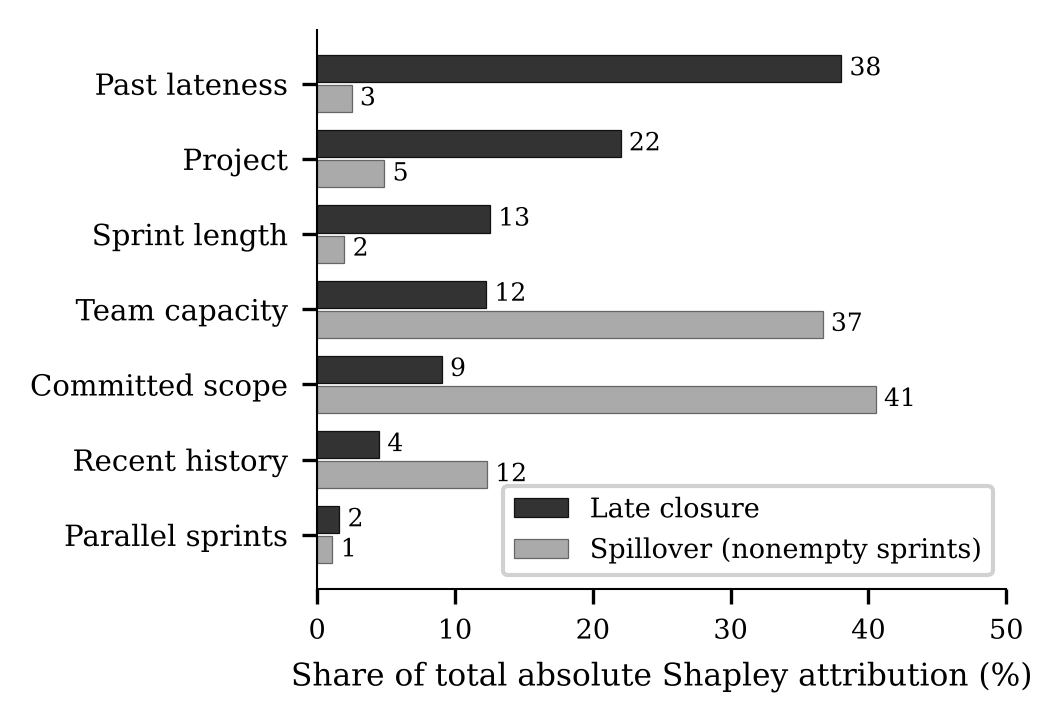
\includegraphics[width=0.85\columnwidth]{fig2_shapley.png}
\caption{Share of mean absolute exact Shapley attribution by feature group for the two random-forest classifiers (strict features), over 150 time-split test sprints.}
\label{fig:shapley}
\end{figure}

\subsection{Numeric Targets}
\label{sec:num}

Issues completed is mostly arithmetic. Committed issues times the team's recent completion rate gives a mean absolute error of 2.10 issues ($R^2$ 0.42); the best learned model, a booster trained on absolute error, manages 1.96 ($R^2$ 0.46), a difference whose interval grazes zero (row 13). Carry share is all but unpredictable ($R^2$ near zero for every model), though that booster trims the error from 0.232 to 0.201 (row 14). Days late gains little, 2.48 against the training median's 2.66. Sprints planned heaviest relative to capacity carry over just 3.2 percentage points more of their scope than the lightest quartile (interval $-2.3$ to $+8.4$), so the data give no support to cutting scope as advice.

\subsection{In-Sprint Early Warning}

Table~\ref{tab:insprint} shows what progress buys. Over planning features alone it buys a great deal for spillover: on the time split gradient boosting moves from 0.830 to 0.926 at 25\%, 0.957 at 50\% and 0.953 at 75\%, each gain with an interval clear of zero. Almost all of it is counting. The number of committed issues still open, with no model, scores 0.925, 0.945 and 0.954 on the time split (row 20), and across projects it beats the model at every checkpoint (0.876, 0.902 and 0.938 against 0.860, 0.897 and 0.927). The share-based rule we first chose as the baseline (0.667, 0.767, 0.802) was the wrong comparator for a label that asks whether any issue stays open. For carry share, one minus the share done so far (0.165, 0.115, 0.064 mean absolute error) matches the model with progress (0.146, 0.112, 0.070) from halfway on.

Late closure barely moves. Gradient boosting scores 0.751 on planning features and 0.754, 0.760, 0.749 and 0.704 with progress at the four checkpoints. Of 24 paired comparisons with the same model without progress, 22 intervals include zero and the other two gains are under 0.03 AUC; on MariaDB the mid-sprint gain is +0.019 (interval $-$0.050 to 0.089). The open-count rule hovers near 0.5. At 50\% the explanations agree: progress takes 34\% of the spillover attribution but only 6\% of the late-closure one, where past lateness still holds 37\%.

\subsection{Leakage Case Studies}
\label{sec:leak}

We reproduce two mistakes on our own data with our first study's legacy logistic regression, scoring F1 at the fixed threshold before and after each. Feed in the sprint's own completion ratio, known only once the sprint is over, and spillover F1 jumps from 0.756 to 0.991 and AUC from 0.834 to 1.000, because the feature restates the label; late closure hardly moves (+0.010), since finishing the work is not what decides when somebody clicks ``complete sprint''. Run SMOTE over the whole pool before splitting and late-closure F1 inflates from 0.457 to 0.646, as synthetic copies of test sprints leak into training, while spillover is untouched at 94\% positives. A third mistake is shuffling sprints before splitting: over five repeats, shuffled 70/30 splits give late closure 0.765 $\pm$ 0.017 against 0.696 $\pm$ 0.054 in time order; spillover hardly moves (0.813 against 0.806). The same mistake can cost a great deal on one outcome and nothing on the other, so each label needs its own audit.

\section{Threats to Validity}

\textbf{Construct.} Jira's completion timestamp marks when a sprint was closed, not when its work was done, so late closure is an administrative event. Spillover says only that at least one committed item went unresolved, which at 94\% prevalence makes it close to a function of scope.

\textbf{Reconstruction.} Replaying the change log beats trusting a static export, but what was never recorded cannot be recovered, and Section~\ref{sec:prov} shows how the story-point fallback caps the spillover estimate. The exact start instant puts many quickly loaded sprints in the empty group. We read completion from each issue's final resolution date, which fails in Confluence Cloud and possibly Confluence Server, and counts a reopened issue at its later resolution.

\textbf{Evaluation.} Eight projects make for wide cluster intervals, and percentile intervals over eight clusters can undercover, so we treat them as exploratory. The timing-confound rerun is a separate implementation. We ran no decision-utility analysis, and the drift within projects means any deployed model would need local recalibration. The Shapley values describe the fitted models, not causes.

\textbf{External.} Every project here is open-source, and the outside checks add two sources and ten projects, with spillover testable in only four of them. Enterprise teams that close sprints on schedule may behave differently.

\balance

\section{Conclusion}

This study contributes an audit more than a tool. Rebuilding the sprint-start state from the change log is not new \cite{r19}; logging where it falls back on static values, and checking each result against the simplest rule, is where the value lies. Under that audit, late closure is a team-habit outcome: planning-time features rank it at about 0.70 AUC over repeated time splits, past lateness and project identity take 60\% of the forest's attribution, progress adds little, and transfer to outside projects is weak. Spillover as a yes-or-no label is close to mechanical: the committed count ranks it at 0.881 at planning and the open count at 0.945 mid-sprint, matching or beating our models. The parallel-sprint timing fix matters for validity, not accuracy; once separated from the features added with it, it does not raise AUC. The lessons are about data and evaluation: rebuild the state at the prediction time, drop the sprints that commit nothing, keep time order, audit leakage one label at a time, and compare every model with a count.

For a team this gives one narrow thing. A team's own late-closure record ranks its next sprints moderately well, as a ranking with a locally set threshold, not as calibrated odds. Future work should replace the spillover label with carry share or a size-normalised threshold, fix the resolution-date defect, and test whether acting on any score improves delivery, which needs a prospective or controlled study.

Every result runs off seed 42 under Python 3.13, scikit-learn 1.8 (1.9 for the outside checks, repeated splits and the reviewer checks), pandas 2.2 and XGBoost 3.1. The artifact at \url{https://github.com/hani-ziad/SwEng_202610} holds the data export, the code, 50 automated tests and every result file behind these numbers.

\begin{thebibliography}{19}
\bibitem{r1} M. Choetkiertikul, H. K. Dam, T. Tran, T. Pham, A. Ghose, and T. Menzies, ``A deep learning model for estimating story points,'' IEEE Trans. Softw. Eng., vol. 45, no. 7, pp. 637--656, Jul. 2019.
\bibitem{r2} S. Porru, A. Murgia, S. Demeyer, M. Marchesi, and R. Tonelli, ``Estimating story points from issue reports,'' in Proc. 12th Int. Conf. Predictive Models Data Analytics Softw. Eng. (PROMISE), 2016, pp. 1--10.
\bibitem{r3} V. Tawosi, R. Moussa, and F. Sarro, ``Agile effort estimation: Have we solved the problem yet? Insights from a replication study,'' IEEE Trans. Softw. Eng., vol. 49, no. 4, pp. 2677--2697, Apr. 2023.
\bibitem{r4} M. Choetkiertikul, P. Banyongrakkul, C. Ragkhitwetsagul, S. Tuarob, H. K. Dam, and T. Sunetnanta, ``Sprint2Vec: A deep characterization of sprints in iterative software development,'' IEEE Trans. Softw. Eng., vol. 51, no. 1, pp. 220--242, Jan. 2025.
\bibitem{r5} P. Hearty, N. Fenton, D. Marquez, and M. Neil, ``Predicting project velocity in XP using a learning dynamic Bayesian network model,'' IEEE Trans. Softw. Eng., vol. 35, no. 1, pp. 124--137, Jan. 2009.
\bibitem{r19} M. Choetkiertikul, H. K. Dam, T. Tran, A. Ghose, and J. Grundy, ``Predicting delivery capability in iterative software development,'' IEEE Trans. Softw. Eng., vol. 44, no. 6, pp. 551--573, Jun. 2018.
\bibitem{r7} Y. J. Pérez Castillo, S. D. Orantes Jiménez, and P. O. Letelier Torres, ``Sprint management in Agile approach: Progress and velocity evaluation applying machine learning,'' Information, vol. 15, no. 11, Art. no. 726, 2024.
\bibitem{r8} P. G. Obike, V. E. Ekong, and O. U. Obot, ``A novel scoring-based Agile sprint deliverability prediction and prioritization using machine learning,'' Int. J. Comput. Appl., vol. 187, no. 49, pp. 40--53, Oct. 2025.
\bibitem{r15} N. V. Chawla, K. W. Bowyer, L. O. Hall, and W. P. Kegelmeyer, ``SMOTE: Synthetic minority over-sampling technique,'' J. Artif. Intell. Res., vol. 16, pp. 321--357, 2002.
\bibitem{r9} S. M. Lundberg and S.-I. Lee, ``A unified approach to interpreting model predictions,'' in Proc. Adv. Neural Inf. Process. Syst. 30, 2017, pp. 4765--4774.
\bibitem{r11} J. Jiarpakdee, C. Tantithamthavorn, and A. E. Hassan, ``The impact of correlated metrics on the interpretation of defect models,'' IEEE Trans. Softw. Eng., vol. 47, no. 2, pp. 320--331, Feb. 2021.
\bibitem{r10} C. Molnar, Interpretable Machine Learning, 2nd ed., 2022. [Online]. Available: \url{https://christophm.github.io/interpretable-ml-book/}
\bibitem{r12} I. Teinemaa, M. Dumas, M. La Rosa, and F. M. Maggi, ``Outcome-oriented predictive process monitoring: Review and benchmark,'' ACM Trans. Knowl. Discov. Data, vol. 13, no. 2, Art. no. 17, 2019.
\bibitem{r13} S. A. Fahrenkrog-Petersen, N. Tax, I. Teinemaa, M. Dumas, M. de Leoni, F. M. Maggi, and M. Weidlich, ``Fire now, fire later: Alarm-based systems for prescriptive process monitoring,'' Knowl. Inf. Syst., vol. 64, no. 2, pp. 559--587, 2022.
\bibitem{r6} V. Tawosi, A. Al-Subaihin, R. Moussa, and F. Sarro, ``A versatile dataset of agile open source software projects,'' in Proc. 19th Int. Conf. Mining Softw. Repositories (MSR), 2022, pp. 707--711.
\bibitem{r17} L. Breiman, ``Random forests,'' Mach. Learn., vol. 45, no. 1, pp. 5--32, 2001.
\bibitem{r18} F. Pedregosa et al., ``Scikit-learn: Machine learning in Python,'' J. Mach. Learn. Res., vol. 12, pp. 2825--2830, 2011.
\bibitem{r16} T. Chen and C. Guestrin, ``XGBoost: A scalable tree boosting system,'' in Proc. 22nd ACM SIGKDD Int. Conf. Knowl. Discovery Data Mining, 2016, pp. 785--794.
\bibitem{r14} J. Gama, I. \v{Z}liobait\.{e}, A. Bifet, M. Pechenizkiy, and A. Bouchachia, ``A survey on concept drift adaptation,'' ACM Comput. Surv., vol. 46, no. 4, Art. no. 44, 2014.
\end{thebibliography}

\end{document}
